\chapter{Ръководство за потребителя}

	\section{Стартиране на системата}
	
	Системата е разделена на два основни компонента и всеки от тях може да бъде стартиран на отделно устройство или на едно - общо такова.
	
	\subsection{Сървър}
	
	Сървърната част е проектирана за разполагане върху мощен компютър. За тестови цели, тя може да се преведе в изпълнение и на по-слаби машини.
	
	\subsubsection{Процес на разполагане}
	
	Системата е предвидена за мултиплатформена употреба, но за целите на дипломната работа е представен метод за разполагане върху \emph{Ubuntu Server\footnote{\url{http://www.ubuntu.com/server}}}. Предполага се версия \emph{12.04} или по-нова.
	
	За инсталиране на MongoDB се изпълнява следната команда:
	\begin{lstlisting}[style=BashStyle]
    > sudo apt-get install mongodb-server
	\end{lstlisting}
	
	\emph{Ubuntu} предоставя инсталация на \emph{Python} по подразбиране. За добавяне на допълнителни модули се използва \emph{pip\footnote{\url{https://pypi.python.org/pypi/pip/}}}. За инсталацията му се изпълнява следната команда в терминала:
	\begin{lstlisting}[style=BashStyle]
    > sudo apt-get install python-pip
	\end{lstlisting}

	Допълнителите модули се добавят с помощта на \emph{pip} чрез следните команди:
	\begin{lstlisting}[style=BashStyle]
    > sudo pip install behave
    > sudo pip install mongoengine
    > sudo pip install bottle
	\end{lstlisting}

	Изпълнение на тестовете предоставя начин за проверка за това дали всичко необходимо е инсталирано правилно. В терминала, текущата директория се променя на \emph{features}, която е поддиректория на главната за проекта. Изпълнява се:
	\begin{lstlisting}[style=BashStyle]
    > behave
	\end{lstlisting}		
	
	Примерен изход от тази команда е предоставен на фигура ~\ref{figure:server-test-output}.
	
	Стартиране на уеб приложението става чрез следната команда (изпълнена в главната директория на проекта):
	\begin{lstlisting}[style=BashStyle]
    > python webapp.py
	\end{lstlisting}		
	
	\begin{figure}[htbp]
		\centering
 		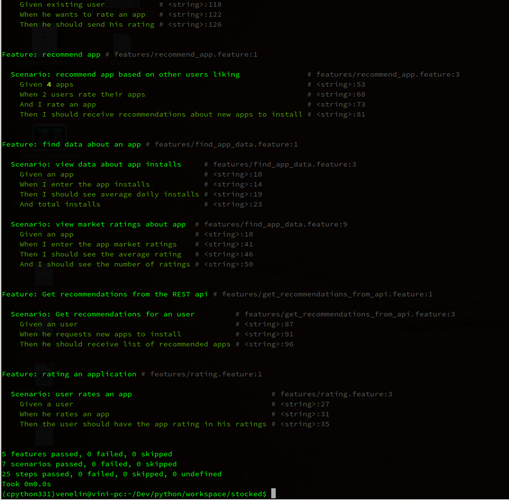
\includegraphics[scale=0.8]{assets/server-test-output.png}
		\caption{Примерен изход от провеждане на тест на сървърната част}
		\label{figure:server-test-output}
	\end{figure}
		
	\subsection{Клиент}
	
	Клиентската част използва \emph{Android SDK}. Подробни инструкции за инсталацията му са дадени на официалния сайт\footnote{\url{http://developer.android.com/sdk/}}. То се използва за пакетиране на мобилното приложение. Апликацията се стартира по стандартния начин за всички подобни приложения и работи върху емулатор и реални устройства. За правилната му работа е необходима свързаност между сървъра и клиента. Стартирано, приложението е показано на фигура ~\ref{figure:client-recommendations}.

	\begin{figure}[htbp]
		\centering
 		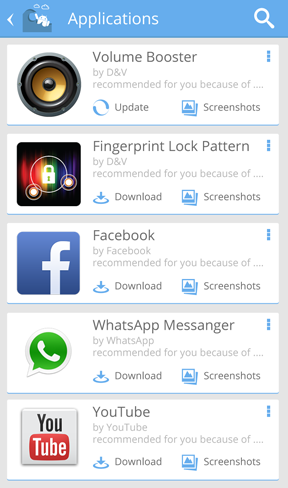
\includegraphics{assets/tsunapper-app-recommendations.png}
		\caption{Примерен поглед върху клиентското приложение}
		\label{figure:client-recommendations}
	\end{figure}